\section{LLVM}
LLVM is an umbrella project that provides a collection of tools for developing low-level
toolchains, e.g assemblers, compilers, debuggers, linkers etc. It is designed to be reusable and
applicable to arbitrary programming languages and target architectures. It started as a
research project at the University of Illinois in 2000 and is widely used today by hobbyists
and professionals alike. There are LLVM frontends for languages such as Haskell, Rust,
Swift and Ruby. Clang is also a part of the LLVM project and built upon
the LLVM toolchain. It provides a compiler, debugger and standard library implementation
for the C language family (C, C++, Objective-C, OpenCL, Cuda etc).

% http://www.rubymotion.com/tour/features/
% https://ghc.haskell.org/trac/ghc/wiki/Commentary/Compiler/Backends/LLVM
% http://llvm.org/ https://en.wikipedia.org/wiki/Clang


\subsection{Overview of LLVM}

% http://www.aosabook.org/en/llvm.html
LLVM is designed to be modular. A compiler written on top of LLVM will in general consist
of three phases; The front-end, the mid-end (also called optimizer), and the back-end
(also known as code generator). The front-end is responsible for lexical and syntatical
analysis of the source code. The mid-end is responsible for target-indenpendent optimizations
and the back-end handles platform specific tasks such as instruction selection, register
allocation and instruction scheduling. The point of LLVM is that the interface between
these modules are well-defined and thus allow for reuse so that, e.g, a front-end for
C uses the same optimizer as a front-end for Rust. In a similar manner the back-end
for x86 and the back-end for ARM uses the same mid-end. See figure \ref{fig:three_phase_compiler}.
LLVM can thus be seen as a \textit{collection of libraries} that perform, or at least
assists in performing, these different tasks.

\begin{figure}[h]
	\centering
	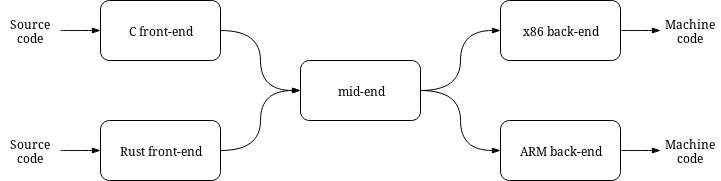
\includegraphics[width=12cm]{background/figures/three_phase_compiler}
	\caption{Three-phase compiler construction. The mid-end is somtimes called an \textit{optimizer}
	and the back-end a \textit{code generator}}
	\label{fig:three_phase_compiler}
\end{figure}

In the case of LLVM, the interface between the front-end and the mid-end is known as the
LLVM IR (\textit{Intermediate Representation}) and is a strongly typed, RISC-like virtual
instruction set that abstracts some details about the machine, such as function call
conventions and registers. To implement a programming language one would then only have to
implement a front-end, that is translate the source code to LLVM IR. One could then pick
and choose from the already existing LLVM optimizer passes and LLVM back-end implementations
to complete the compiler.

Only the back-end is of concern to this thesis, so it will focus exclusively on that.

\subsubsection{LLVM Machine Representation}

To represent machine specific IR LLVM uses the LLVM MIR (\textit{Machine Intermediate Representation}),
which is a human readable, YAML serialized format that is used to test code generation passes
in LLVM. That is, if we stop LLVM prematurely we can view the current progress in the form
of an LLVM MIR. For example, the iterative factorial function written in C:

\lstinputlisting[language=C,tabsize=2,frame=single,breaklines=true,showstringspaces=false,
backgroundcolor= \color{lightgray}]
{background/examples/factorial.c}

gets translated to the following MIR when targeting the Hexagon V4 architecture and
terminating after instruction selection, right before register allocation and instruction
scheduling.

\lstinputlisting[tabsize=2,frame=single,breaklines=true,showstringspaces=false,
backgroundcolor= \color{lightgray}]
{background/examples/factorial.mir}

Courtesy of the Unison documentation for the code examples.
% https://github.com/unison-code/unison/tree/master/doc/code

\subsection{LLVM back-end}

% https://llvm.org/docs/WritingAnLLVMBackend.html
The LLVM back-end is responsible for three main tasks: Intruction selection, register
allocation and instruction scheduling. They are performed mostly in isolation to each
other, which simplifies the architecture but introduces some interesting challenges.

The general behaviour of an LLVM back-end is that it transforms LLVM IR to machine code
for a specific target platform. Exactly what it produces is depended on the target architecture
but it is common to generate assembly corresponding to the instruction set of the target
machine.

\subsubsection{Instruction selection}


\subsubsection{Register Allocation}
% Mention the problem with offset and having to scavenge register
% https://youtu.be/objxlZg01D0?t=48m53s

\subsubsection{Instruction Scheduling}
